%%%%%%%%%%%%%%%%%%%%%%%%%%  phdsymp_sample2e.tex %%%%%%%%%%%%%%%%%%%%%%%%%%%%%%
%% changes for phdsymp.cls marked with !PN
%% except all occ. of phdsymp.sty changed phdsymp.cls
%%%%%%%%%%                                                       %%%%%%%%%%%%%
%%%%%%%%%%    More information: see the header of phdsymp.cls   %%%%%%%%%%%%%
%%%%%%%%%%                                                       %%%%%%%%%%%%%
%%%%%%%%%%%%%%%%%%%%%%%%%%%%%%%%%%%%%%%%%%%%%%%%%%%%%%%%%%%%%%%%%%%%%%%%%%%%%%%


%\documentclass[10pt]{phdsymp} %!PN
\documentclass[twocolumn]{phdsymp} %!PN
%\documentclass[12pt,draft]{phdsymp} %!PN
%\documentstyle[twocolumn]{phdsymp}
%\documentstyle[12pt,twoside,draft]{phdsymp}
%\documentstyle[9pt,twocolumn,technote,twoside]{phdsymp}

\usepackage[english]{babel}       % Voor nederlandstalige hyphenatie (woordsplitsing)

\usepackage{graphicx}                   % Om figuren te kunnen verwerken
\usepackage{graphics}			% Om figuren te verwerken.
\graphicspath{{fig/}}               % De plaats waar latex zijn figuren gaat halen.

\usepackage{times}

\hyphenation{si-mu-la-ted re-a-lis-tic packets really in-clu-ding}

\def\BibTeX{{\rm B\kern-.05em{\sc i\kern-.025em b}\kern-.08em
    T\kern-.1667em\lower.7ex\hbox{E}\kern-.125emX}}

\newtheorem{theorem}{Theorem}

\begin{document}

\title{A privacy-friendly recommender system\\ for mobile devices} %!PN

\author{Thorwald Frederik Lambrecht}

\supervisor{Marleen Denert, Luc Martens, Toon De Pessemier}

\maketitle

\begin{abstract}
This article tries to create the ideal privacy-friendly recommender system for a mobile device. In doing so it will strive to extend the limits of the trade-off between privacy, accuracy and performance existing in recommender systems. To achieve this the solution will be based on  homomorphic encryption.
\end{abstract}

\begin{keywords}
Privacy, mobile, recommender
\end{keywords}

\section{Introduction}
\PARstart{T}{o} allow personalised recommendations, recommender systems need to access privacy-sensitive data from their users. This allows the service provider to retain the data and opens the door for privacy breaches. The privacy breaches, aside from those due to a dishonest provider or a gullible user, could also be due to a lack of data protection from attackers.\\ There are several approaches to improve the privacy of the user. First and foremost the user could be better educated about the extent his data is kept and used. Secondly, the law could also be more strict concerning the issue. Another option is the use of privacy-friendly algorithms. \\
The use of the existing solutions however decreases at least either the accuracy of the recommendations or the performance. Considering the mobile formfactor, it is also important to have an approach that does not require a lot of processortime or data transmission by the client. To see how there could be created a mobile recommender system that would tackle the trade-off, research in existing privacy-friendly solutions was needed. 

\section{Research in privacy-friendly recommendation algorithms}
There are multiple existing methods to increase privacy in recommender systems. These methods include methods using anonimisation, randomisation, aggregation of userprofiles and cryptographic protocols. For each of these we took an indepth look in at least one example and made a comparison.\\The solution based on anonimisation \cite{anonimisatie} makes use of agents that communicate anonymously. Even though during requests and the comparison of users' preferences the users themselves stay anonym, anonymity does not guarantee privacy as proven by Narayan \cite{anon}.\\The randomisation algorithm used by Polat and Du \cite{rand} does not provide full privacy either as the server can still know in what range the user rated his items, plus it loses accuracy drastically when using small datasets. However this approach does not demand a lot of work at the clientside and does not lose much accuracy.\\  The use of aggregation of userprofiles by Shokri et al. in \cite{agg} offers the users the deniability of their preferences but still shows the server their real ratings. It also has a decent accuracy.\\ A solution with cryptographic protocols with a peer-to-peer character does reach high privacy levels but needs a social network where users are online. This method requires too much computation on the clientside.\\ The best bet seems to be the solution using cryptographic protocols and two servers by Erkin et al \cite{dyn}. This approach based on an earlier solution \cite{erkin} delivers the best privacy and does not require a lot of computations by the clients. In this regard the cryptographic protocols in this paper were chosen to serve as a start for this solution.

\section{The privacy-friendly solution}
For our solution we decided to create a native android application and the servers are made in the programming language JAVA. They interact all by the HTTP-protocol. As database we used the MovieLens database with 100.000 ratings, 943 users and 1682 items. The solution in \cite{dyn} uses two servers, a recommender server and a second server that is deployed by a trusted third party. The client sends his ratings and preferences to the recommenderserver encrypted by the public Paillierkey of the second server. This does not have to take place literally every time he rates an item. To generate a prediction score for an item communication is needed between the Paillier and DGK cryptosystems on both servers to sum and count the encrypted ratings of like-minded users. The like-minded users are calculated by the known Pearson-correlation, which is partly computated by the client. For the computations on the serverside for the Pearson-correlation it uses complicated protocols between the two servers like a multiplicationprotocol and a thresholdprotocol. There are several practical decisions that needed to be taken when implementing these protocols, especially on the userside. As opposed to \cite{dyn} the user should not send his encrypted ratings individually. This would enable the recommenderserver to know he just rated an item. An option is to choose several random items and include encrypted zero-values for these. However the items could randomly all be chosen in a particular field and thus giving the service provider information. This could be avoided by choosing these items in a smart way, but this leaves values like his preferences and offsets calculated by an old mean. To have optimal privacy in our application the user sends his ratings and preferences, also called his profile, in one time, with encrypted zero values for all items that aren't rated. For this solution it is necessary that per rating there is another bit encrypted by the user added to his profile. This encrypted bit $ q_{U_x,i} $ that is 1 if the user x has rated the item i and 0 if not. This makes it possible to count the number of effectively rated items used in our formula (\ref{stdrecom}). The encryption of the values is also best calculated the moment the user sends his profile. Otherwise the server could see which encrypted values are changed. In the original paper \cite{dyn} calculates a prediction by taking the average value of the ratings for that item from users that score a similarityvalue above a thresholdvalue. However the protocols used allow an improvement by generating predictions based on a version of a formula used often in user-user collaborative filtering:
\begin{equation}\label{stdrecom}p_{U_1,i} = \bar{r}_{U_1} + \frac{\sum_{j=2}^{n}(r_{(U_j,i)} - \bar{r}_{U_j}).s_{(U_1,U_j)}.q_{(U_j,i)}}{\sum_{j=2}^{n} s_{(U_1,U_j)}.q_{(U_j,i)} }
\end{equation}
where $r_{(U_x,i)}$ denotes the rating value for user x for item i, $\bar{r}_{U_x}$ the average over all items for user x and $p_{U_1,i}$ denotes the prediction from user 1 for item i.
Here the value $s_{(U_1,U_j)}$ stands for the bit that is calculated by the thesholdprotocol and this bit is 1 if the user has a similarity above the thresholdvalue. In stead of the ratingvalue itself, the user now sends the encrypted offset from his average $\bar{r}_{U_1}$. This value has to be converted to a positive integer for the use of the cryptosystems. This can happen in an easy way $result = ((r_{(U_j,i)} - \bar{r}_{U_j})+5)*1000$. Once the sum is taken over all the similar users, the client can revert the conversion by division through 1000 and subtracting 5 per similar user.

\section{Results}
The predictions of the improved method (the light line)  shows significant better scores for accuracy than the method from \cite{dyn} (the dark line). 

\begin{figure}[ht]
\begin{center}
	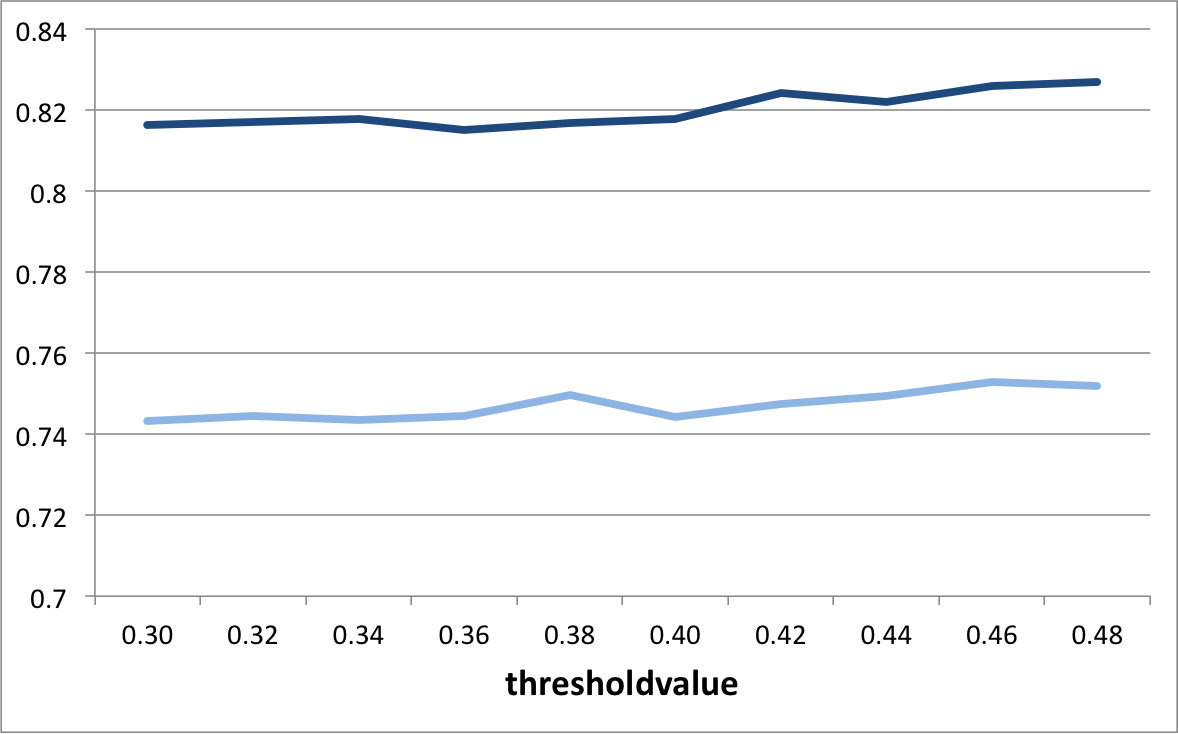
\includegraphics[width=.40\textwidth]{mae}
	\caption{MAE results over 10.000 predictions over different thresholdvalues}
\end{center}
\end{figure}
\begin{figure}[ht]
\begin{center}
	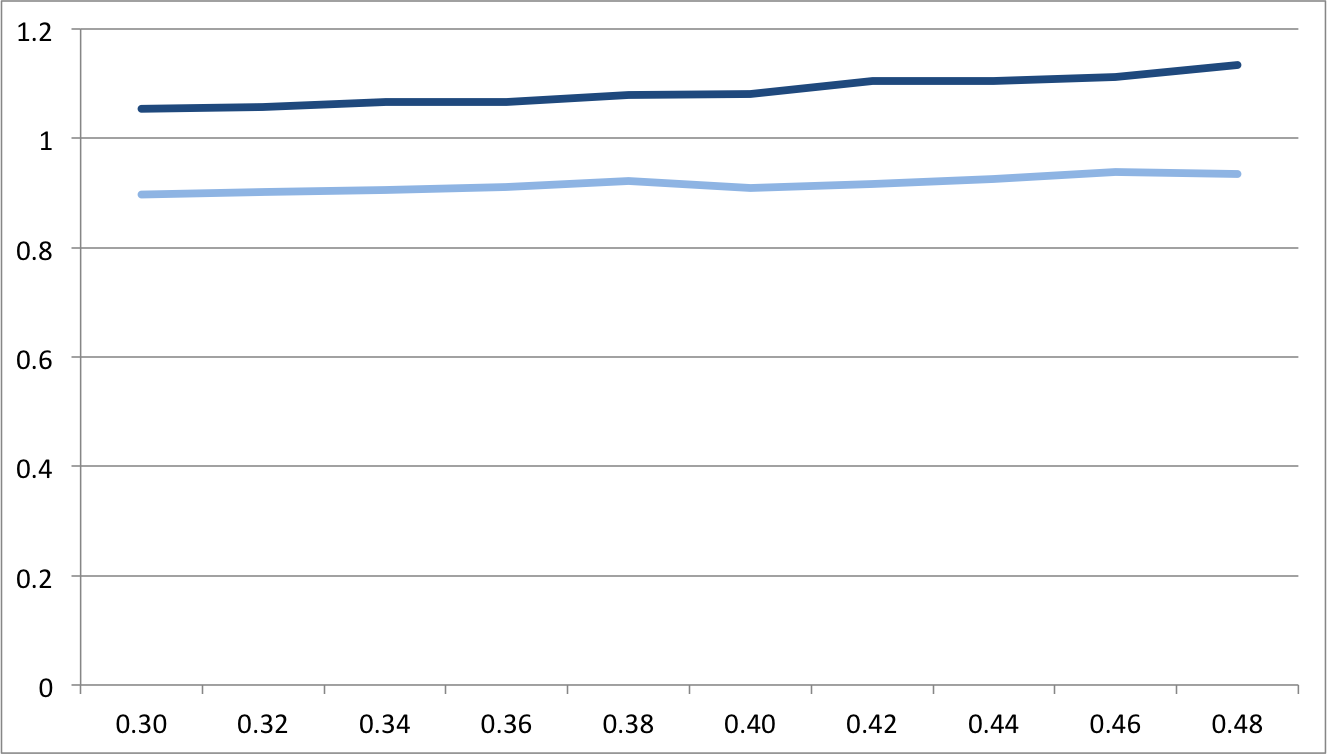
\includegraphics[width=.40\textwidth]{mse}
	\caption{MSE results over 10.000 predictions over different thresholdvalues}
\end{center}
\end{figure}

The MAE improved from around 0.82 to around 0.74, this is very close to the MAE of a privacy-unfriendly solution on the same database by \cite{rand} which is 0.7146. Since the privacy is unchanged our solution still obtains very high privacy levels. The performance on our mobile device is $O(N+S)$ with N as number of items and S as number of preferences. This contains the encryption of a userprofile and thus for each item 2 encryptions and for each preference 1 encryption was done by our testtablet \footnote{Samsung Galaxy Tab4 (7.0) Wi-Fi on Android 4.4.2} in 1,52 seconds averaged over 10 times. The servers engage in heavy computation, it took our testserver\footnote{MacBook Pro 4 GB RAM 2.4 GHZ i7 processor} 7 minutes 26 seconds to generate predictions for all 1682 items for one user, when using 30 preferences. This however can still be optimized with the use of a lower-level protocol as it was, looking back, not the best choice of using the HTTP-protocol for the communication between the two servers. Also the user could send less values to the server at once as discussed. This would have an impact on the accuracy of the algorithm but would decrease the work at the serverside and the size of its' database.

 
\section{Conclusion}

The solution provided guarantees a very high level of privacy by the use of encryption with Paillier and DGK and the fact that the server does not know which items are rated by the user. It also offers high accuracy scores without a lot of computation on the clientside. These properties make it ideal for use as a recommender for mobile devices. The servers themselves have to engage in heavy computation but this computation could be further optimized.








\nocite{*}
\bibliographystyle{phdsymp}
%%%%%\bibliography{bib-file}  % commented if *.bbl file included, as
%%%%%see below


%%%%%%%%%%%%%%%%% BIBLIOGRAPHY IN THE LaTeX file !!!!! %%%%%%%%%%%%%%%%%%%%%%%%
%% This is nothing else than the phdsymp_sample2e.bbl file that you would%%
%% obtain with BibTeX: you do not need to send around the *.bbl file        
%%
%%---------------------------------------------------------------------------%%
%
\begin{thebibliography}{1}
\bibitem{anonimisatie}

Ciss{\'e}e, Richard and Albayrak, Sahin
\newblock {\em An Agent-based Approach for Privacy-preserving Recommender Systems},
\newblock Proceedings of the 6th International Joint Conference on Autonomous Agents and Multiagent Systems,2007

\bibitem{anon}
Narayanan, Arvind and Shmatikov, Vitaly
\newblock{\em Robust De-anonymization of Large Sparse Datasets},
\newblock Proceedings of the 2008 IEEE Symposium on Security and Privacy, 2008

\bibitem{rand}
Polat, Huseyin and Du, Wenliang
\newblock{\em SVD-based Collaborative Filtering with Privacy},
\newblock Proceedings of the 2005 ACM Symposium on Applied Computing,2005


\bibitem{agg}
Shokri, Reza and Pedarsani, Pedram and Theodorakopoulos, George and Hubaux, Jean-Pierre
\newblock{\em Preserving {P}rivacy in {C}ollaborative {F}iltering
                 through {D}istributed {A}ggregation of {O}ffline
                 {P}rofiles},
\newblock{The 3rd {ACM} {C}onference on {R}ecommender {S}ystems ({R}ec{S}ys), 2009}

\bibitem{dyn}
Zekeriya Erkin and Thijs Veugen and R.L. Lagendijk
\newblock{\em Privacy-Preserving Recommender Systems in Dynamic Environments},
\newblock IEEE Workshop on Information Forensics and Security, 2013

\bibitem{erkin}
Zekeriya Erkin and Michael Beye and Thijs Veugen and Reginald L. Lagendijk
\newblock{\em Efficiently computing private recommendations},
\newblock ICASSP,2011


\end{thebibliography}
%
%%---------------------------------------------------------------------------%%

\end{document}

%%%%%%%%%%%%%%%%%%%%%  End of phdsymp_sample2e.tex  %%%%%%%%%%%%%%%%%%%%%%%%%%%
